\begin{figure}[htbp]
  \begin{tabular}{ccc}
    \begin{minipage}{0.33\hsize}
      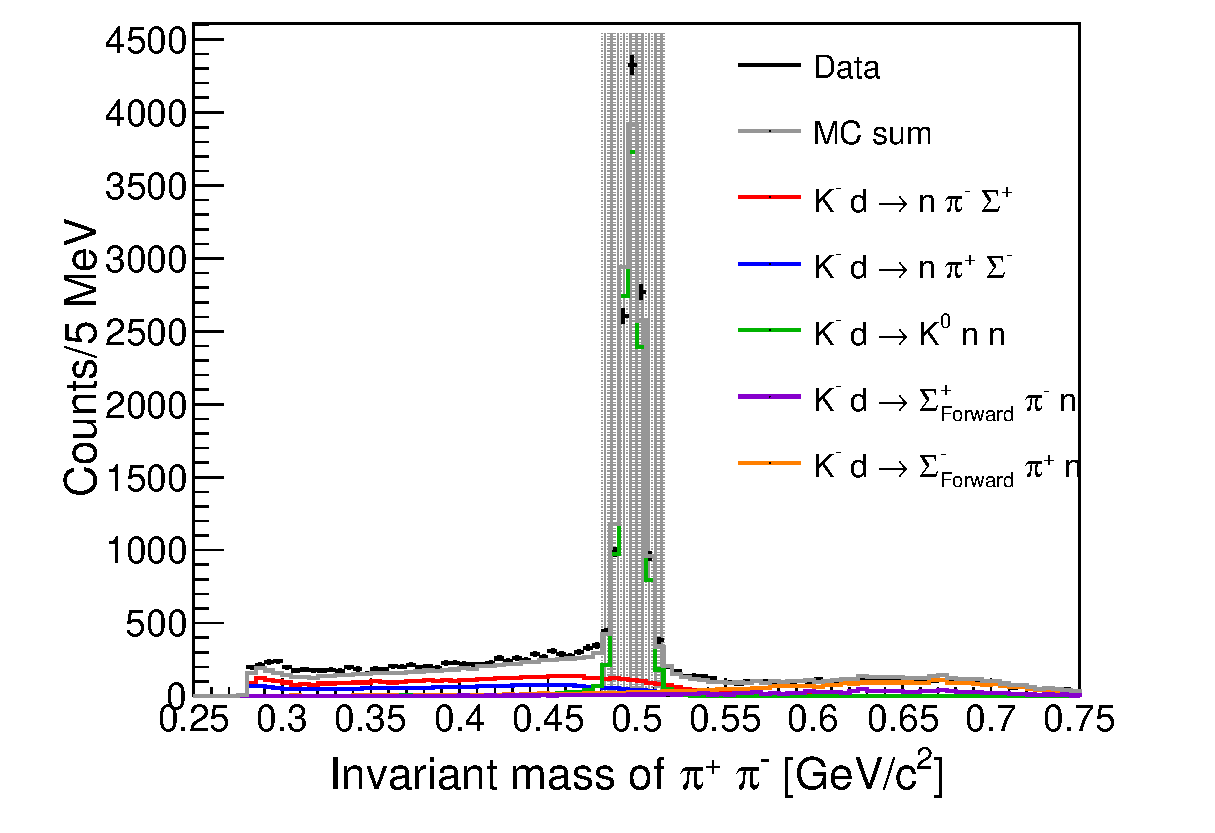
\includegraphics[width=4cm]{../pic/Dron/KN_ana/IM_pipi.eps}
    \end{minipage}
    \begin{minipage}{0.33\hsize}
      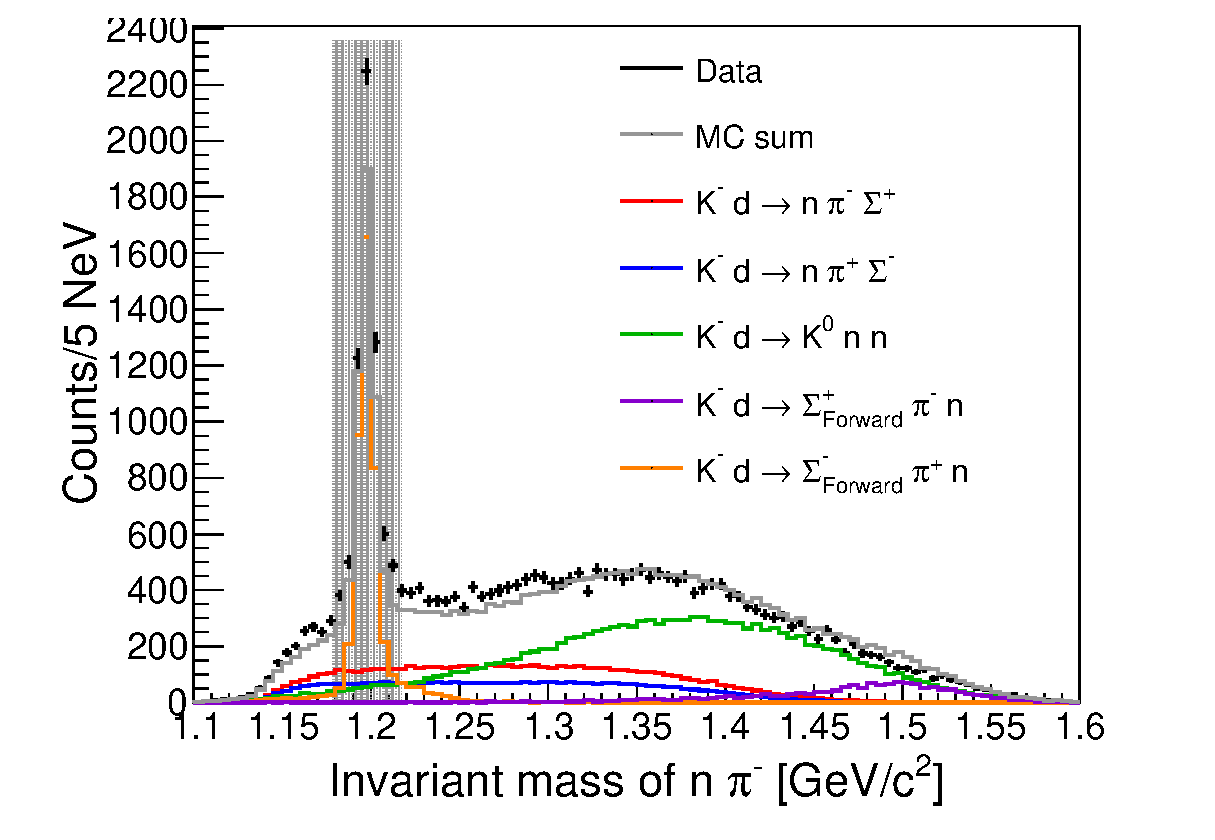
\includegraphics[width=4cm]{../pic/Dron/KN_ana/IM_npim.eps}
    \end{minipage}
    \begin{minipage}{0.33\hsize}
      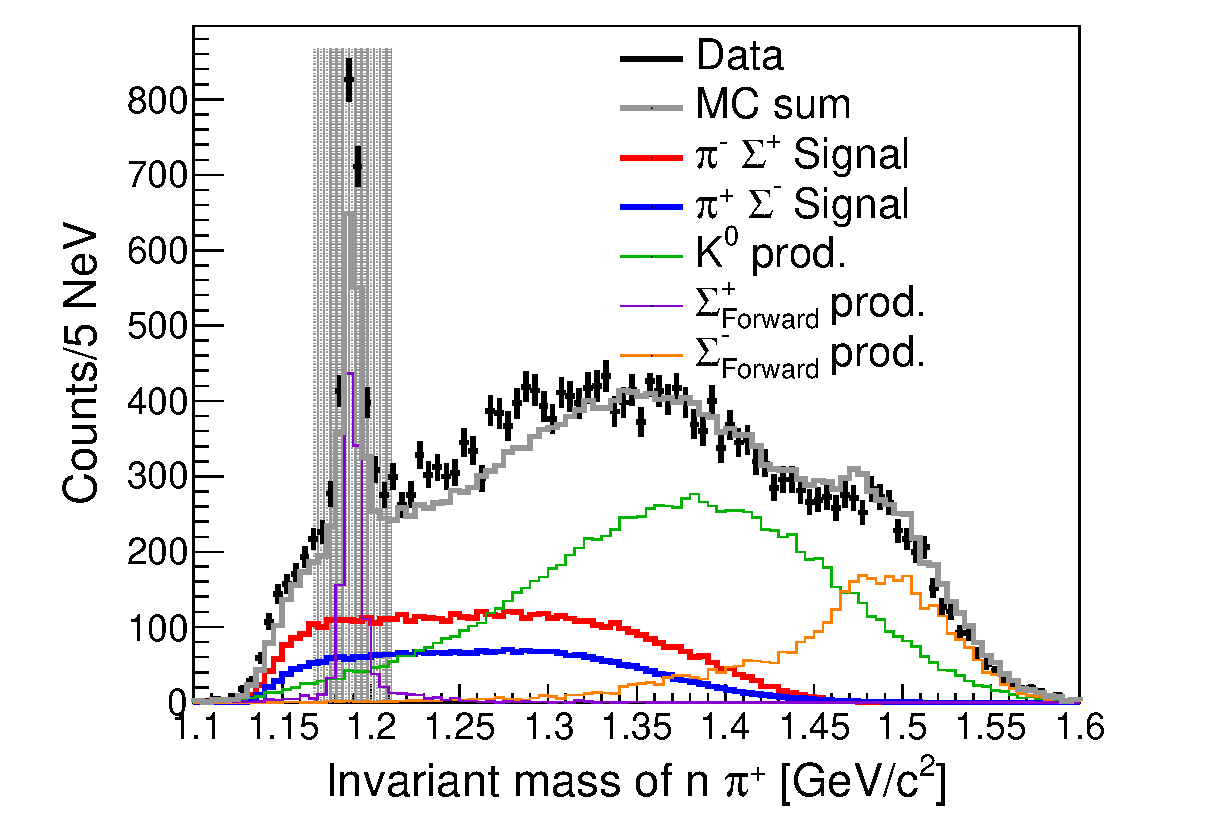
\includegraphics[width=4cm]{../pic/Dron/KN_ana/IM_npip.eps}
    \end{minipage}
  \end{tabular}

  \caption{
    The figures show template fitting for background estimation.
    The right, center, and left figures show invariant masses of $\pi^+ \pi^-$, $n \pi^-$ and $n \pi^+$, respectively.
    Error bars represent data spectra.
    Bold lines indicate the backward $\pi \Sigma$ production signals: red for $\pi^-\Sigma^+$ and blue for $\pi^+\Sigma^-$.
    Thin green, purple, and orange lines represent the $K^0$, $\Sigma^-_{forward}$ and $\Sigma^+_{forward}$ production reactions, respectively.
    Gray lines show the sum of the Monte Carlo simulations.
    Gray hatched areas indicate the 3$\sigma$ rejection regions estimated by fitting with a Gaussian function and a polynomial background.
  }
  \label{fig:fit_IM}
\end{figure}
